\chapter{Prototype}\label{wo6}

\section{Database}\label{wo6_1}

\begin{center}
	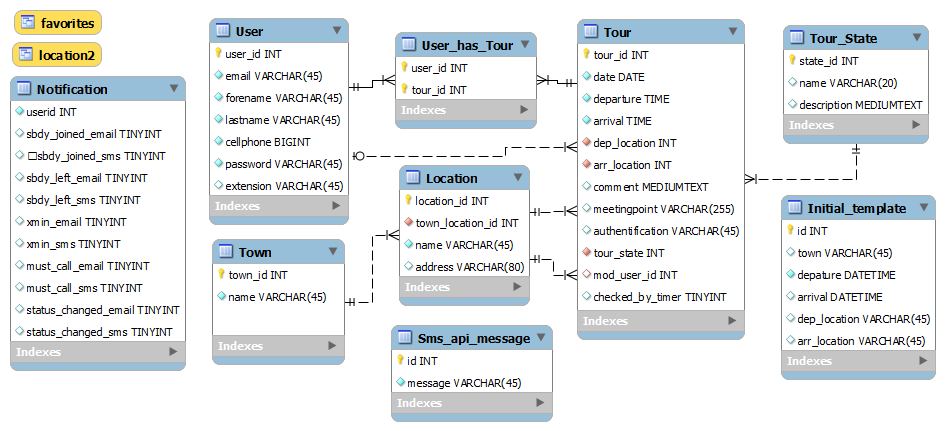
\includegraphics[width=17cm]{img/Datenbank_Model}
\end{center}

\section{Architecture}\label{wo6_2}

\begin{center}
	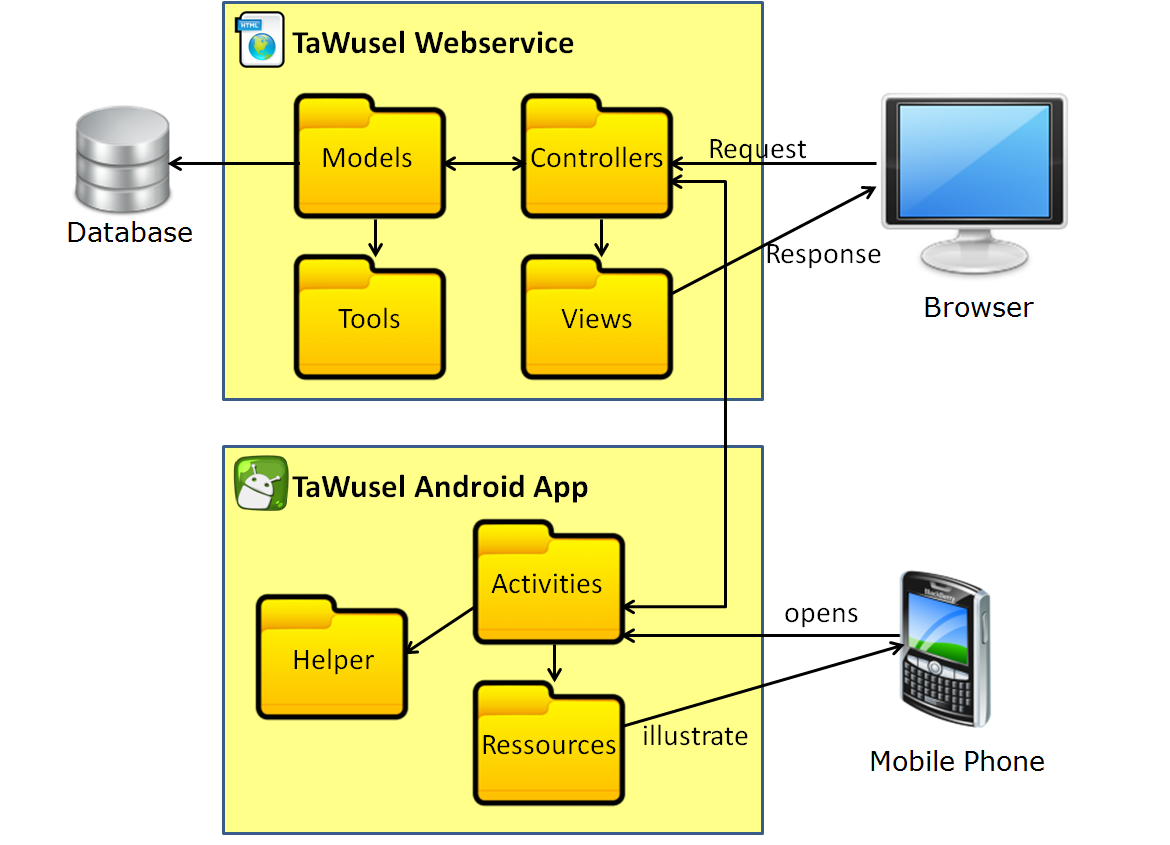
\includegraphics[width=17cm]{img/Architekturdiagramm}
\end{center}


\section{Installation guide - web-application}\label{wo6_3}

\textbf{1.} Grab play from http://www.playframework.org/ and install it.

\textbf{1.1.} Basically it is: unzip, add to \$PATH and run it. Or follow these instructions:
http://www.playframework.org/documentation/2.0.2/Installing\\
\textbf{2.} Set up a mysql-database for this project, e.g.:

CREATE DATABASE tawusel; GRANT ALL ON tawusel.* TO tawusel@localhost IDENTIFIED BY 'pass'; (if you want to use other credentials,
change file conf/application.conf accordingly)\\
\textbf{3.} In the project's root folder (i.e. here) run play run\\

Point web browser to http://localhost:9000/

\section{Installation guide - Android-application}\label{wo6_4}

\textbf{1.} Make sure you locate the tawusel.properties into the assets folder. Here you have to replace the json server
property ("http://10.0.2.2:9000/") by the address of the server your tawusel service is running on.\\
\textbf{2.} Generate your tawusel.apk.\\
\textbf{3.} Install the apk on your mobile phone.\\
(remark: the current version works stable on android 2.3.3 but its working on higher versions is not guaranteed)
